\documentclass[11pt,a4paper]{article}
\usepackage[margin=3cm]{geometry}
\usepackage[english]{babel}
\usepackage[dvipsnames]{xcolor}
\usepackage[utf8x]{inputenc}
\usepackage{amsmath}
\usepackage{graphicx}
\setlength {\marginparwidth }{2cm}
\usepackage[colorinlistoftodos]{todonotes}
\usepackage{setspace}
\usepackage{etoolbox}
\usepackage{framed,color}
\usepackage{tcolorbox}
\usepackage[english]{babel}
\usepackage[nottoc]{tocbibind}
\usepackage{float}
\usepackage{pdfpages}
\renewcommand{\baselinestretch}{1.3}

\begin{document}

\begin{titlepage}

\newcommand{\HRule}{\rule{\linewidth}{0.5mm}} % Defines a new command for the horizontal lines, change thickness here

\center % Center everything on the page

%----------------------------------------------------------------------------------------
%	HEADING SECTIONS
%----------------------------------------------------------------------------------------

\textsc{\LARGE New Zealand}\\[0.5cm]

\textsc{\LARGE  Maritime School}\\[1.5cm]
\textsc{\Large ETO Course 942.465}\\[0.2cm] % Major heading such as course name
\textsc{\large Shipboard Maintenance and Repair Procedures – Electrotech}\\[0.5cm] % Minor heading such as course title

%----------------------------------------------------------------------------------------light
%	TITLE SECTION
%----------------------------------------------------------------------------------------

\HRule \\[0.5cm]
{ \huge \bfseries Module Assignment}\\[0.2cm] % Title of your document
\HRule \\[0.5cm]
\begin{minipage}{0.4\textwidth}
\begin{flushleft} \large
\emph{Author:}\\
Levi \textsc{Dubbelman}

\textit{SN: 190000929}\par
\end{flushleft}
\end{minipage}
~
\begin{minipage}{0.4\textwidth}
\begin{flushright} \large
\emph{Supervisors:} \\
John \textsc{Lamb} \&

Nick \textsc{Cossar}
\end{flushright}
\end{minipage}\\[2cm]
{\large May, 2019}\\[2cm]

\includegraphics[width=4cm]{logo.png}
\vfill

\end{titlepage}

\tableofcontents
\newpage
% BEGINNING OF LEARNING OUTCOME 1
\section{Learning Outcome 1}
\begin{tcolorbox}[colback=red!5!white,colframe=red!75!black,title=\textbf{Demonstrate ability to use lubrication and cleaning materials and equipment}]
With an emphasis on electrical systems and machinery, write an explanation (approximately 200 words) including diagrams and any other related information for each of the following:
\begin{itemize}
\item Selects correct lubricating products for applications.
\item Cleaning products are selected and used appropriately.
\end{itemize}
\end{tcolorbox}
\subsection{Selects correct lubricating products for applications.}
Lubrication is extremely important to prevent mechanical damage when two metal surfaces are interacting. The majority of bearings are specifically greased as to not need any lubrication during their lifespan. For electrical equipment, a teflon or silicon-based grease may be used. These materials must be:
\begin{itemize}
\item Non Conductive

Conductive greases may short circuit electrical equipment
\item Water-repelling

Water and moisture ingress must be limited to ensure efficient operation
\item Immune to salt-water

Salt water is both conductive and may remove other greases. It is important to protect against it at sea.
\item Non flammable (or very high flash point)

Flammable greases may combust as friction temperatures may be very high
\item Rust/corrosion preventing

Rust and corrosion may cause mechanical damage.
\end{itemize}
Silicone and teflon-based lubricants are often used by consumers in applications where other common consumer lubricants, such as petroleum jelly, would damage certain products, such as insulation. They have extremely high dieletric strength, and water resistance.
\subsection{Cleaning products are selected and used appropriately.}
To increase operating efficiency of electrical equipment, a degreaser is used. This will remove grease, oil, tar, adhesives, dirt, grime, corrosion or sludge machinery. It is important that the product used is \textbf{NOT}:
\begin{itemize}
\item Corrosive

Corrosive cleaners will damage sensitive electrical components, or erode away any electrical insulation, such as PVC on wires.
\item Flammable

Flammable or products with low flash points may create a fire hazard during normal operation of the device, as temperatures internally may exceed 60-70 degrees C.
\item Conductive

Conductive products will create a short circuit, which will burn out any motors.
\end{itemize}
An example of a suitable electrical cleaner is the CRC Lectra Clean, which fits the criteria for acceptable materials. In addition, this product evaporates quickly, leaving little to no residue within the machine, and has a dielectric strength of 50,000V.
\begin{center}
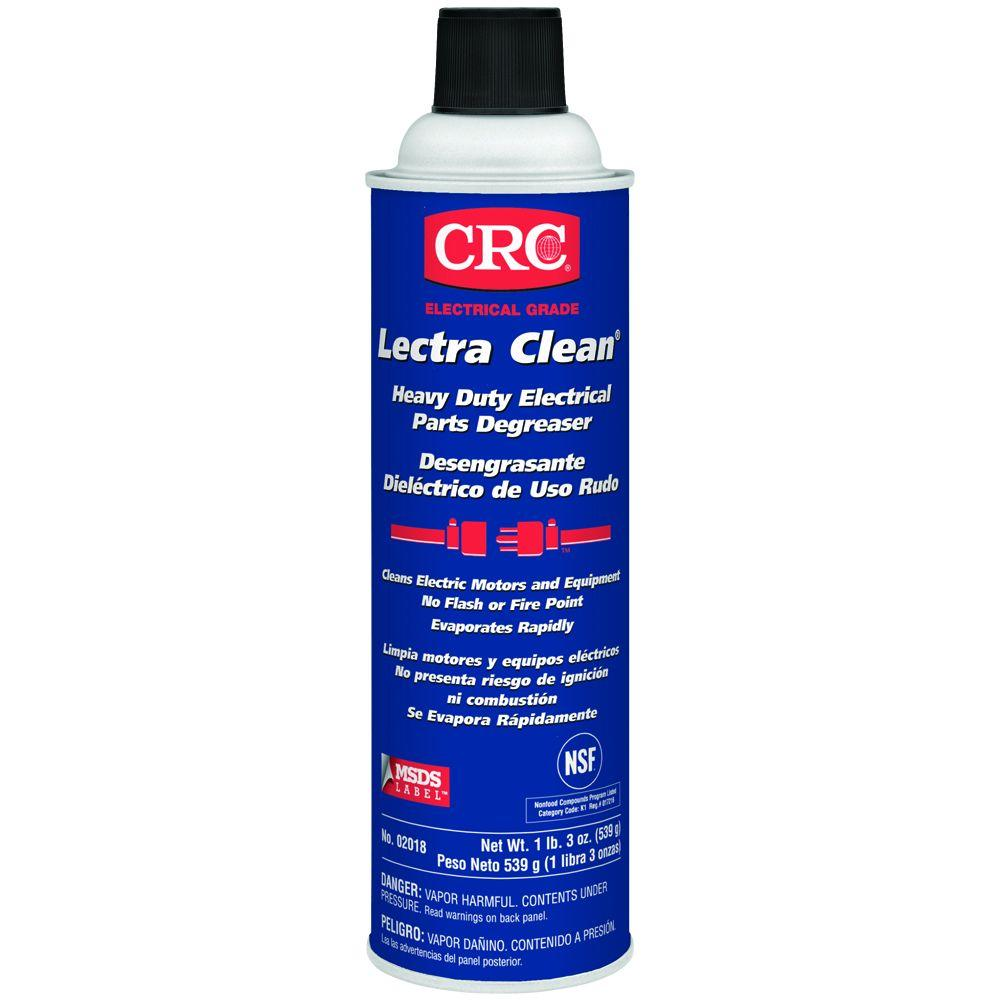
\includegraphics[width=10cm]{electroclean}
\end{center}
However, this particular product is damaging to plastics, and is therefore not suitable on electrical equipment with a large amount of plastics, such as printed circuit boards, or sensitive components.
\newpage
% BEGINNING OF LEARNING OUTCOME 2
\section{Learning Outcome 2}
\begin{tcolorbox}[colback=red!5!white,colframe=red!75!black,title=\textbf{Demonstrate knowledge of safe disposal of waste materials}]
Interprets International Convention for the Prevention of Pollution from Ships, technical annexes I to IV of MARPOL.
With an emphasis on electrical systems and machinery, write an explanation (approximately 200 words) including diagrams and any other related information for each of the following:
\begin{itemize}
\item Oily Water Separators.
\item Grey Water Systems.
\item Sewerage Treatment Systems.
Guidelines and information can be found in the Aurora and Diamond Princess Ships manuals. It is important to detail the product water overboard discharge characteristics and alarms used to prevent marine pollution from these systems.
\end{itemize}
\end{tcolorbox}
\subsection{Oily Water Separators}
The purpose of a shipboard oily water separator is to separate oil and other contaminants that could be harmful for the oceans. They are most commonly found on board ships where they are used to separate oil from oily waste water such as bilge water before the waste water is discharged into the environment. These discharges of waste water must comply with the requirements laid out in Marpol 73/78.

All OWS equipment can separate oil and water, do so automatically, and produce clean water for discharge overboard that contains no more than 15 parts per million oil.

The most common form of OWS is the gravity plate separator. A gravity plate separator contains a series of oleophilic plates through which the contaminated water flows. The oil in the water coalesces on the underside of the plate eventually forming droplets before coalescing into liquid oil which floats off the plates and accumulates at the top of the chamber. The oil accumulating at the top is then transferred to waste oil tank on the vessel where it is later discharged to a treatment facility shore side.
\begin{center}
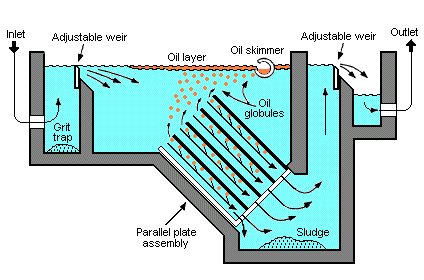
\includegraphics[width=12cm]{oil}\par
A Gravity Plate Separator diagram.
\end{center}
\subsection{Grey Water Systems}
Greywater or sullage is all wastewater generated on ship without fecal or petroleum contamination, i.e. all streams except for the wastewater from toilets or sumps. Sources of greywater include, sinks, showers, baths, clothes washing machines or dish washers. As greywater contains fewer pathogens than domestic wastewater, it is generally safer to handle and easier to treat and reuse on ship for toilet flushing, cooling,, and other non-potable uses. Under MARPOL there are no regulations involving greywater, other than the regulations which overlap from other discharge regulations, e.g. oil parts-per-million and sulfide content. Most ships with an excess simply discharge the greywater into the ocean.

This is not an issue on the relatively small amount of greywater discharge from vessels with reasonably low crew numbers, such as cargo or offshore. However, on cruise ships especially, where passengers number in the thousands, and the laundry/galley are constantly producing a high volume of greywater, this is becoming an issue. MARPOL regulations will likely be updated to reflect this in the coming few years.

Regardless, ships will still use tools for measuring impurities onboard ship, especially oil, to ensure that their greywater discharge complies with the lax regulations.
\subsection{Sewerage Treatment Systems}
Discarding sewage is heavily regulated under MARPOL. To avoid heavy fines, sewage must be disposed of safely. This can either be done at port, or at sea if treated. However, keeping sewage for any great length of time creates a terrible smell, and may simply be better to treat the sewage and then discharge into the sea. This is done with a Sewage treatment plant. The most preferred type of sewage treatment plant is that involving aerobic bacteria. This system can be divided into three parts:
\begin{itemize}
\item Aeration chamber

 This chamber is fed with raw sewage which has been grounded to form small particles. The advantage of breaking sewage in small particles is that it increases the area and a high number of bacteria can attack simultaneously to decompose the sewage. The sewage is decomposed into carbon dioxide, water, and inorganic sewage. The air is forced through the diffuser into the air chamber. The pressure of air flow also plays an important role in decomposition of the sewage. If the pressure is kept high then the mixture of air and sewage will not take place properly and it will escape without doing any work required for decomposition. It is for this reason; controlled pressure is important inside the sewage treatment plant as this will help in proper mixing and decomposition by the agitation caused by air bubbles. Generally, the pressure is kept around 0.3-0.4 bars.

 \item Settling tank

The mixture of liquid and sludge is passed to settling tank from the aeration chamber. In the settling tank, the sludge settles at the bottom and clear liquid on the top. The sludge present at the bottom is not allowed to be kept inside the settling tank as this will lead to the growth of anaerobic bacteria and foul gasses will be produced. The sludge formed is recycled with the incoming sludge where it will mix with the later and assist in the breakdown of sewage.

\item Chlorination and Collection

In this chamber, the clear liquid produced from the settling tank is overflown and the liquid is disinfected with the help of chlorine. This is done because of the presence of the e-Coli bacteria present in the liquid. To reduce these bacteria to acceptable level chlorination is done. Moreover, to reduce the e-Coli, the treated liquid is kept for a period of at least 60 minutes. In some plants, disinfection is also done with the help of ultraviolet radiation. The collected liquid is discharged to overboard or settling tank depending on the geological position of the ship. If the ship is in restricted or near coastline then the sewage will be discharged into the holding tank; otherwise, the sewage is discharged directly into the sea when a high level is reached and is disposed of automatically until low-level switch activates.
\end{itemize}
\newpage
% BEGINNING OF LEARNING OUTCOME 3
\section{Learning Outcome 3}
\begin{tcolorbox}[colback=red!5!white,colframe=red!75!black,title=\textbf{Demonstrate basic understanding of executing routine maintenance and repair procedures}]
With an emphasis on electrical systems and machinery, write an explanation (approximately 200 words) including diagrams and any other related information for the following:
\begin{itemize}
\item Selection and use of appropriate equipment and tools.
\end{itemize}
\end{tcolorbox}
\subsection{EXAMPLE: Repairing an Induction Motor}
With any work done board ship, it must be thoroughly documented. For instance, an S.O.P. (standard operating procedure) for the inspection and repair of an induction motor would be as such:
\begin{enumerate}
\item File a permit-to-work.

This provides evidence that work commenced on that motor. It includes information such as the technician's name, date and time commenced, and the reason why it was commenced.
\item Isolate, Lock Out and Tag Out

Ensuring a motor is completely de-energized is extremely important. Attempting to start the motor is one of the best methods to ensure total disconnection, but also testing using a live-line tester or multimeter (if low voltage). Checking between each phase, and each phase and ground is good practice. Lock out the switch if possible, and tag it with your name to ensure it cannot be re-energized while work is being done.
\item Disconnect and remove

Methodically removing each terminal connection and bolt will ensure an easy lift. Place on a trolleyjack for safe moving. Weights above 25KG should not be lifted by hand.

\item Take measurements

For insulation resistance, an insulation tester, or "megger" is used. This produces a high DC voltage (to measure resistive impedance, otherwise inductive or capacitive impedance will be measured as well) and should be used to check the insulation between each winding, and each winding and ground. A healthy reading will be in the dozens of millions of ohms, or \textit{infinity}, i.e. $>999$ million ohms. This reading tells us there is virtually no electrical connection made. Checking the resistance of each winding is also good practice. This can be done with a multimeter on low ohms. If one winding is dramatically lower than the other two (e.g. $5+$ ohms) it could mean that at some point in the winding there is a breakdown of insulation between wires. For bearings, check that there is no lateral movement. If there is, use a bearing puller and replace it by heating the new bearing on a bearing heater and quickly replacing it.
\end{enumerate}
Once these steps are done, replace the motor and re-bolt it down, being sure to connect each terminal correctly. De-isolate and test the motor, checking for any repetition of the fault. Log this information with the chief engineer or electrician.
\newpage
% BEGINNING OF LEARNING OUTCOME 4
\section{Learning Outcome 4}
\begin{tcolorbox}[colback=red!5!white,colframe=red!75!black,title=\textbf{Demonstrate basic understanding of manufacturer’s safety guidelines and shipboard instructions}]
With an emphasis on electrical systems and machinery, write an explanation (approximately 200 words) including diagrams and any other related information for the following:
\begin{itemize}
\item Maintenance activities are carried out in accordance with technical, safety and procedural specifications.
\end{itemize}
\end{tcolorbox}
\subsection{EXAMPLE: Entering an Azimuth Thruster Space}
With work done with respects to safety guidelines, an example may be to enter a dangerous enclosed space. For this example we'll take the azimuth thruster space.
\begin{center}
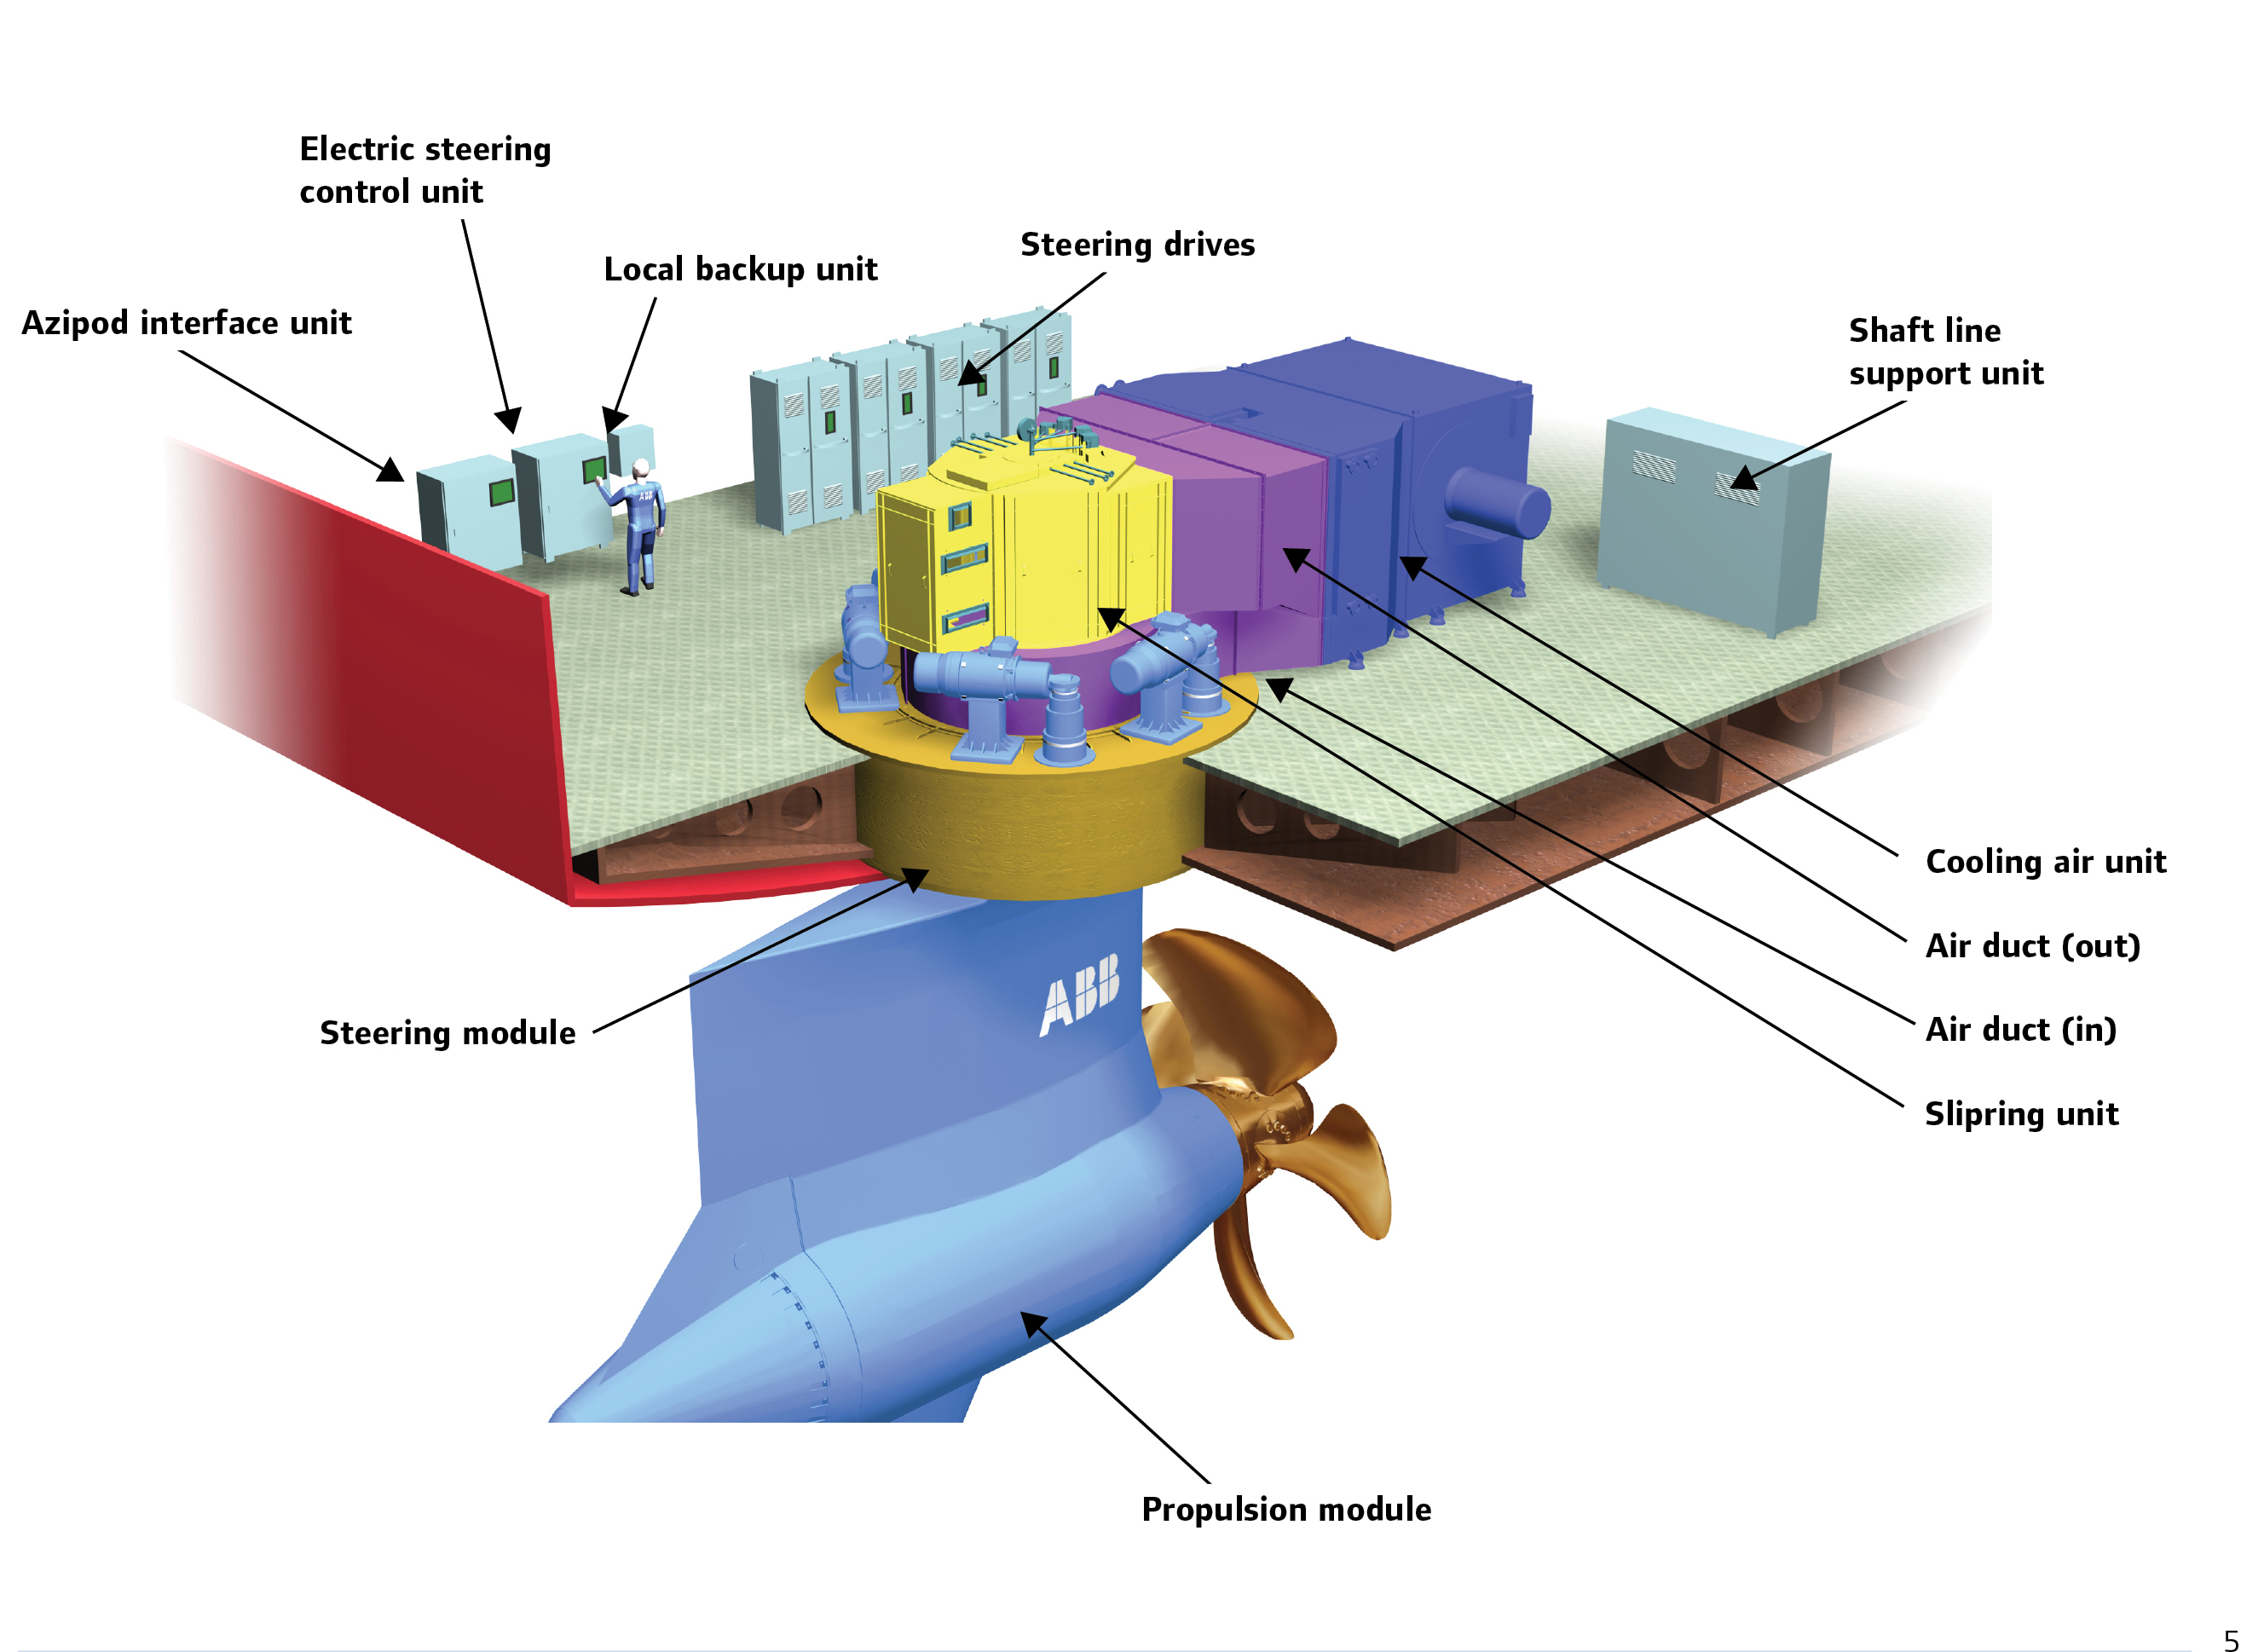
\includegraphics[width=12cm]{ABB}
\end{center}
\begin{enumerate}
\item Drills

Before any actual work is needed to be done in the azimuth thruster space, technical staff should run drills on entering the space and recovering a downed man.
\item Permit to Work

As with any work to be done, a permit to work must be filed. In addition to this, an enclosed space permit will also be required. The S.O.P for azimuth thruster spaces will have documented guidelines on how long to ventilate the area before entry. You're also working with high voltage, and should file the relevant permits too.
\item Risk Assessment

Do a risk assessment with your superior. Also involve your master. This will allow you to map out any potential hazards before they become threatening
\item Ventilate

Using forced draft fans if possible, it's important to release any harmful fumes or gas buildups, such as CO2.
\item Harness

Some overalls will be fitted with harness straps, if not, don a harness to be lowered into the space. Any additional PPE should be adorned now as well. For example, a hard hat with flashlight may be advantageous
\item Lock Out Tag Out

Isolate the azimuth thruster's transformers and control system, lock them out and tag them so they can't be re-energized. Once down in the space, you may need to engage the lock on the prop to prevent windmilling, especially if working with divers. Also locking the steering gear so the pod cannot rotate while you're inside.
\item Inspect

Run your standard tests as per the SOP. This may include an insulation resistance tester, or simply a multimeter. Be sure to prove that they work before entering the space, and prove them once again after your test to ensure accuracy.
\item Rectify

This is now the time to perform any relevant work, IF that work was expected before entering the space. If you find something in your inspection you weren't expecting, now would be the time to contact your superior. You may need to resurface out of the space.
\item Paperwork

Describe accurately the date at which the work began, why it began,  and exactly what you did while in the space. This helps to ensure the next person to maintain the azimuth thruster understands what has happened in there.
\end{enumerate}
\newpage
% BEGINNING OF LEARNING OUTCOME 5
\section{Learning Outcome 5}
\begin{tcolorbox}[colback=red!5!white,colframe=red!75!black,title=\textbf{Demonstrate knowledge of handling of stores}]
With an emphasis on electrical systems and machinery, write an explanation (approximately 200 words) including diagrams and any other related information for the following:
\begin{itemize}
\item Describe procedures for safe handling, stowage and securing of stores.
\end{itemize}
\end{tcolorbox}
\subsection{EXAMPLE: Ordering Replacement PLC}
On ship, you may be expected to maintain the stock levels and stores of the ship. An example on the procedure for placing a purchase order for a PLC would be as follows:
\begin{enumerate}
\item Confirm stock levels

Don't believe the computer -- confirm for yourself that the stock level is below expected for that unit.
\item Get approval

Do this through your superior -- usually either Chief Engineer or Chief Electrician -- they take responsibility for overstocking
\item Fill out Purchase Order

Ensure you have the right make and model number, the correct quantity, and what port you want to pick the unit up at.
\item Update Head Office

It's not uncommon for head office to be notified automatically when you place the purchase order. If they're not, however, be sure to let them know.
\item Send it away

This is usually done electronically -- by email or automatically through a stock management system.
\item Pick it up

When you arrive at your destination, collect it and sign it onto the system. Update your stock levels so nobody goes and orders another.
\item Place in stores or use

Put the unit in the correct location, sometimes this may be directly in a housing as your last unit in stock had just failed.
\end{enumerate}
\newpage
\end{document}
